\documentclass[preview]{standalone}
\usepackage{tikz}
\begin{document}
  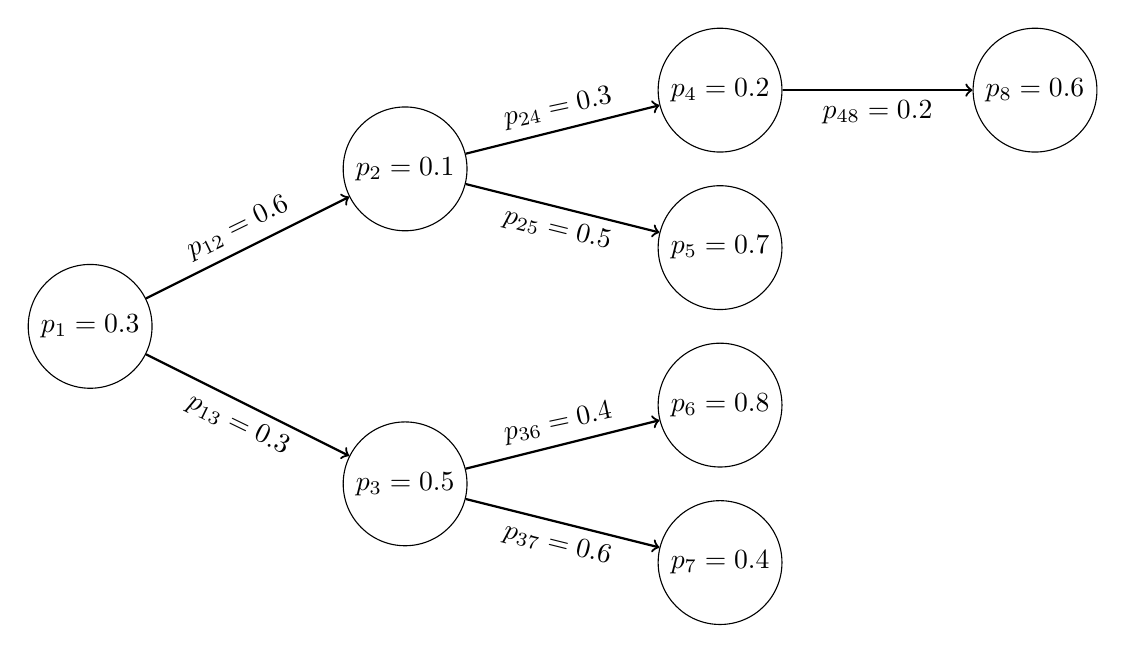
\begin{tikzpicture}[
roundnode/.style={circle, draw=black, minimum size=7mm},
]
%Nodes
\node[roundnode]      at (0,0) (node1) {$p_1=0.3$};
\node[roundnode]      at (4,2) (node2) {$p_2=0.1$};
\node[roundnode]      at (4,-2) (node3) {$p_3=0.5$};
\node[roundnode]      at (8,3) (node4) {$p_4=0.2$};
\node[roundnode]      at (8,1) (node5) {$p_5=0.7$};
\node[roundnode]      at (8,-1) (node6) {$p_6=0.8$};
\node[roundnode]      at (8,-3) (node7) {$p_7=0.4$};
\node[roundnode]      at (12,3) (node8) {$p_8=0.6$};
%Lines
\path[->,draw,thick] (node1) edge node[above, rotate=26] {$p_{12}=0.6$}(node2) ;
\path[->,draw,thick] (node2) edge node[above, rotate=12] {$p_{24}=0.3$}(node4) ;
\path[->,draw,thick] (node2) edge node[below, rotate=346] {$p_{25}=0.5$}(node5) ;
\path[->,draw,thick] (node4) edge node[below] {$p_{48}=0.2$}(node8) ;
\path[->,draw,thick] (node1) edge node[below, rotate=334] {$p_{13}=0.3$}(node3) ;
\path[->,draw,thick] (node3) edge node[above, rotate=12] {$p_{36}=0.4$}(node6) ;
\path[->,draw,thick] (node3) edge node[below, rotate=346] {$p_{37}=0.6$}(node7) ;
\end{tikzpicture}
\end{document}

% convert -density 300 tikz.pdf -quality 90 tikz.png
